\documentclass{beamer}
\usetheme{Warsaw}
\usepackage{beamerthemesplit}
\usepackage{color}
\usepackage{textcomp}
\title{Formatting The Document \\ Using \LaTeX}
\author{SPACE}
\date{\today}
%\logo{
\includegraphics[width=1cm]{space}}
\begin{document}
\maketitle

\begin{frame}{Titles, Chapters, and Sections...}
\begin{itemize}
\pause \item[]\begin{block}{Try this!!}
\begin{itemize}
\pause \item \textbackslash section\{\ldots\}
\pause \item \textbackslash subsection\{\ldots\}
\pause \item \textbackslash subsubsection\{\ldots\}
\pause \item \textbackslash paragraph\{\ldots\}
\pause \item \textbackslash subparagraph\{\ldots\}
\end{itemize}
\end{block}
\pause \item Change to report class
\pause \item[] \begin{block}{Try..}
\begin{itemize}
\pause \item \textbackslash part
\pause \item \textbackslash chapter
\end{itemize}
\end{block}
\end{itemize}
\end{frame}

\begin{frame}{Table of Contents}
\begin{itemize}
\pause \item[] \begin{figure}
\centering
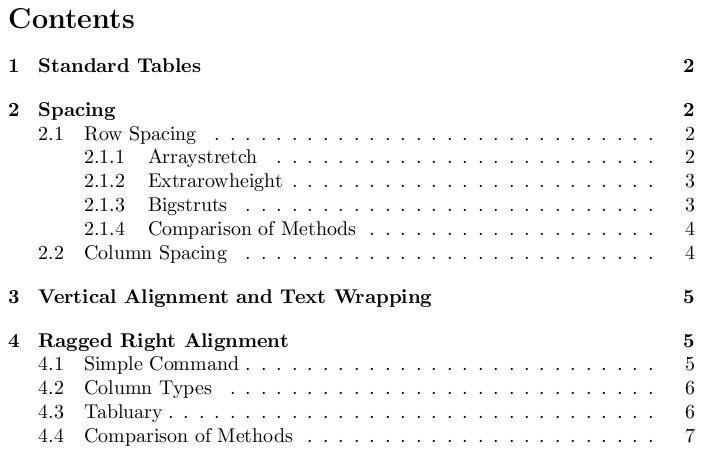
\includegraphics[width=0.7\linewidth,angle=0]{table}
\caption{Table of Contents}
\label{fig:golden}
\end{figure}
\pause\item\framebox{\textbackslash tableofcontents}
\item[] A new document has to be compiled twice or thrice to get a correct table of contents.
\end{itemize}
\end{frame}

\begin{frame}{Starred Versions}
\begin{itemize}
\pause \item All sectioning commands listed above also exist as ``starred'' versions.
\pause \item “starred” version of a command is built by adding a star * after the command
name
\pause \item This generates section headings that do not show up in the table
of contents and are not numbered
\pause \item For Example :
\pause \item[] \textbackslash section\{First Heading\} $\rightarrow$ \textbackslash section*\{First Heading\}
\end{itemize}
\end{frame}

\begin{frame}{Titles}
\begin{itemize}
\pause \item The title of the whole document is generated by issuing the command 
\pause \item[] \centering \framebox{\textbackslash maketitle}
\pause \item The contents of the title have to be defined by the commands
\centering \pause \item[] \framebox{\textbackslash title\{...\},\textbackslash author\{...\} and optionally \textbackslash date\{...\}}
\flushleft \pause \item We can add several Authors by using \textbackslash and.
\end{itemize}
\end{frame}

\begin{frame}{Cross References}
\begin{itemize}
\pause \item In books, reports and articles, there are often cross-references to figures,
tables and special segments of text 
\pause \item \LaTeX provides the following commands for cross referencing 
\pause \item[] \framebox{\textbackslash label\{marker\}, \textbackslash ref\{marker\} and \textbackslash pageref\{marker\}} 
\pause \item where marker is an identifier chosen by the user.
\pause \item \LaTeX ~replaces \textbackslash ref by
the number of the section, subsection, figure, table, or theorem after which the corresponding \textbackslash label command was issued.
\pause \item \textbackslash pageref prints the pagenumber of the page where the \textbackslash label command occurred.
\item[] \textbackslash subsection\{Second \}\textbackslash label\{flower\} $\rightarrow$\textbackslash ref\{flower\}
\item[] Eg:~A reference to this subsection looks like:``see section \textcolor{red}{2.8} on page \textcolor{red}{42}.''
\end{itemize}
\end{frame}

\begin{frame}{Footnotes}
\begin{itemize}
\item A footnote is printed at the foot of the current page
\pause \item[] \textbackslash footnote\{text for footnote\}
\pause \item Footnotes should always be put after the word or sentence they refer to
\pause \item Eg:~ Footnotes \textbackslash footnote\{This is a footnote\}~are often used by people using \LaTeX \\
\item[] 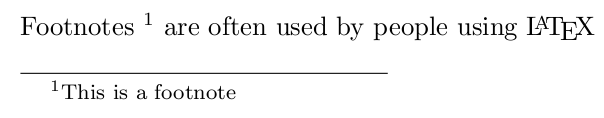
\includegraphics[width=10cm]{footnote}
\end{itemize}
\end{frame}

\begin{frame}{Emphasized Words}
\begin{itemize}
\pause \item If a text is typed using a typewriter, important words are emphasized by \underline{underlining} them
\pause \item[] \framebox{\textbackslash underline\{text\}}
\pause \item In printed books words are emphasized by typesetting them in an italic font
\pause \item[] \framebox{\textbackslash emp\{text\}}
\pause \item[] \begin{block}{Try this\ldots}
\item[] ctrl+b
\item[] ctrl+i
\end{block}
\end{itemize}
\end{frame}

\end{document}